\section{Analiza funkcjonalna systemu}
\subsection{Diagram przypadków użycia}
\begin{figure}[h]
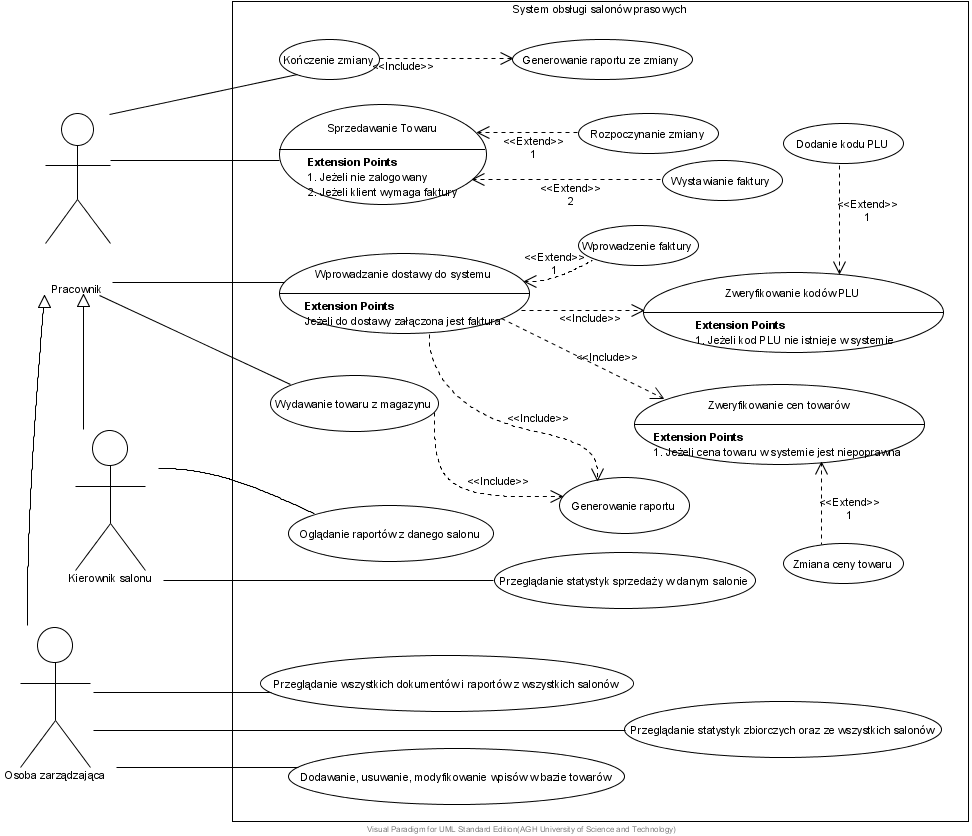
\includegraphics[width=1\textwidth]{gfx/usecase.png}
\caption{Diagram przypadków użycia systemu}
\end{figure}
\clearpage
\subsection{Diagram kontekstowy (przepływu danych - poziom 0)}
\begin{figure}[h]
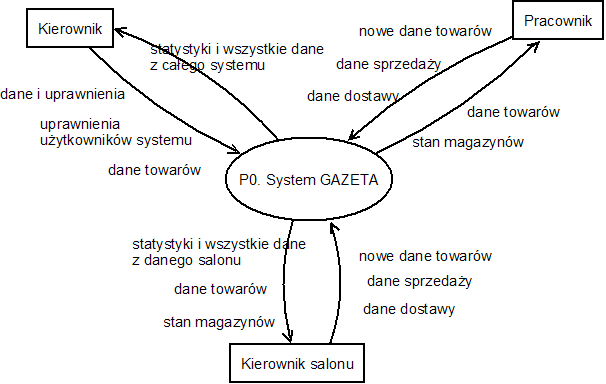
\includegraphics[width=1\textwidth]{gfx/dfd-0.png}
\caption{DFD - poziom 0 (diagram kontekstowy)}
\end{figure}
\clearpage
\subsection{Diagram przepływu danych - poziom 1}
\begin{figure}[h]
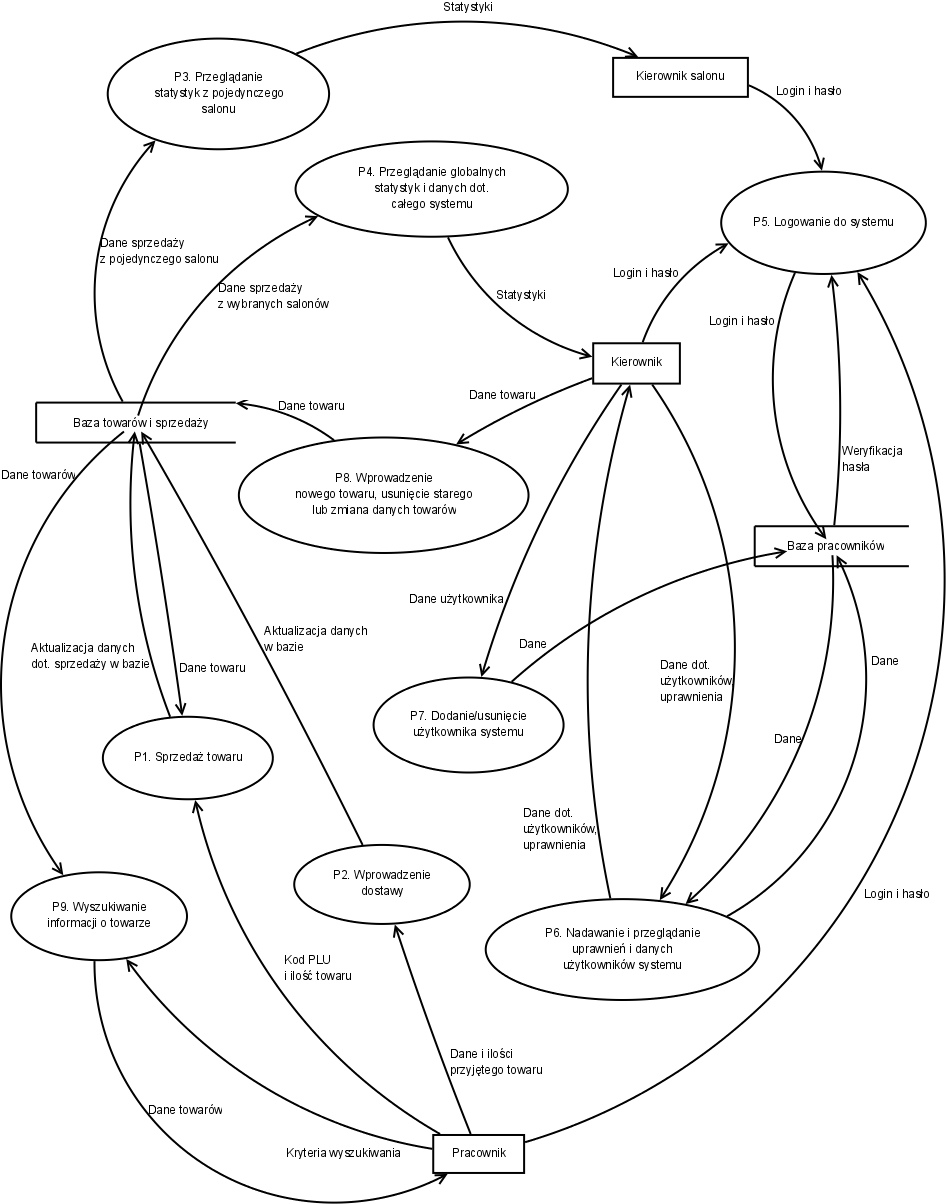
\includegraphics[width=1\textwidth]{gfx/dfd-1.png}
\caption{DFD - poziom 1}
\end{figure}
\clearpage
\subsection{Diagramy przepływu danych - poziom 2}
\subsubsection{Poziom 2.1 - Sprzedaż towaru}
\begin{figure}[h]
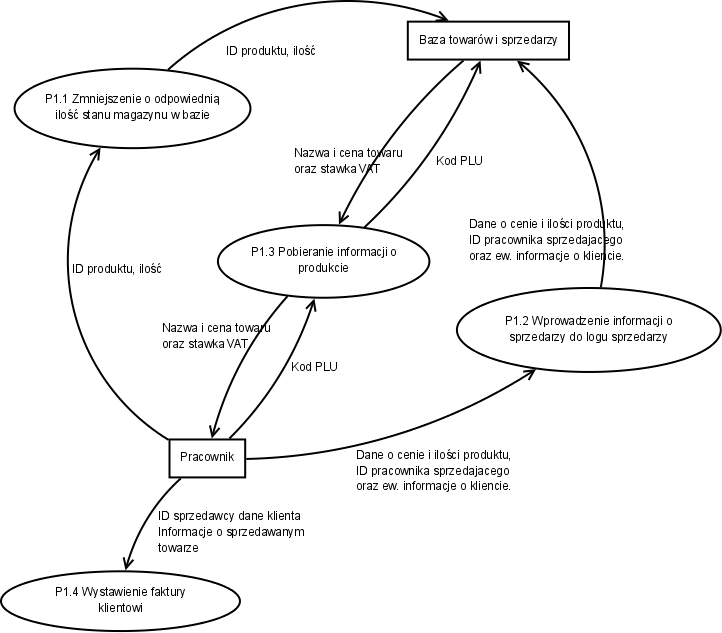
\includegraphics[width=1\textwidth]{gfx/dfd-2-1.png}
\caption{DFD - poziom 2.1 - Sprzedaż towaru}
\end{figure}
\clearpage
\subsubsection{Poziom 2.2 - Wprowadzenie dostawy}
\begin{figure}[h]
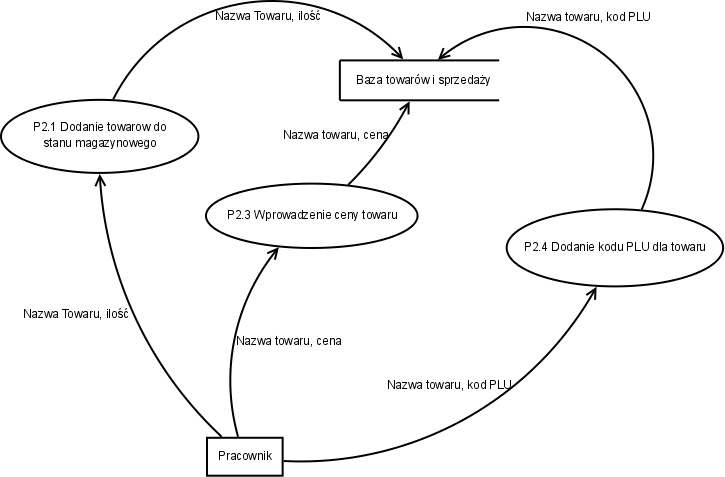
\includegraphics[width=1\textwidth]{gfx/dfd-2-2.png}
\caption{DFD - poziom 2.2 - Wprowadzenie dostawy}
\end{figure}
\clearpage
\subsubsection{Poziom 2.3 - Przeglądanie statystyk salonu}
\begin{figure}[h]
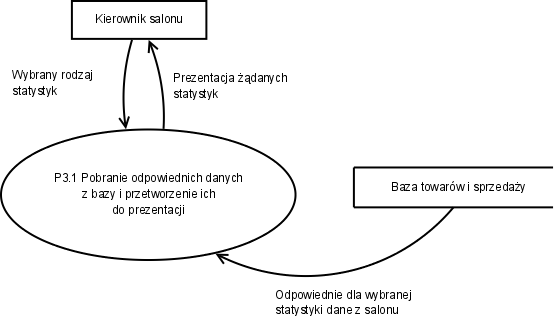
\includegraphics[width=1\textwidth]{gfx/dfd-2-3.png}
\caption{DFD - poziom 2.3 - Przeglądanie statystyk salonu}
\end{figure}
\clearpage
\subsubsection{Poziom 2.4 - Przeglądanie statystyk globalnych}
\begin{figure}[h]
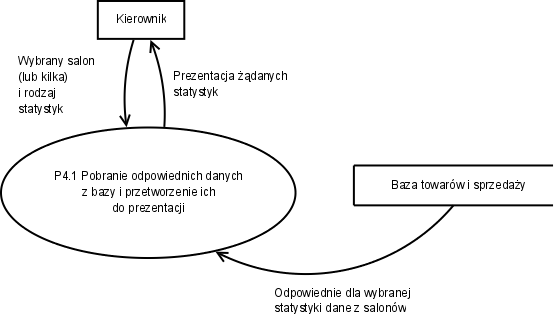
\includegraphics[width=1\textwidth]{gfx/dfd-2-4.png}
\caption{DFD - poziom 2.4 - Przeglądanie statystyk globalnych}
\end{figure}
\clearpage
\subsubsection{Poziom 2.5 - Logowanie do systemu}
\begin{figure}[h]
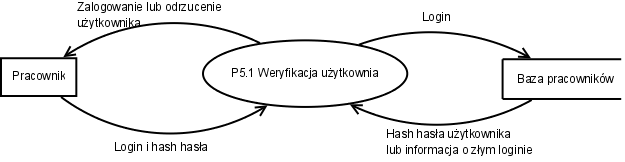
\includegraphics[width=1\textwidth]{gfx/dfd-2-5.png}
\caption{DFD - poziom 2.5 - Logowanie do systemu}
\end{figure}
\clearpage
\subsubsection{Poziom 2.6 - Nadawanie i przeglądanie uprawnień i danych użytkowników systemu}
\begin{figure}[h]
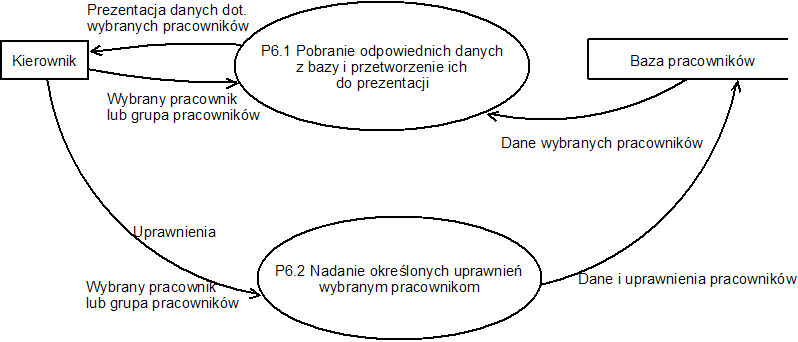
\includegraphics[width=1\textwidth]{gfx/dfd-2-6.png}
\caption{DFD - poziom 2.6 - Nadawanie i przeglądanie uprawnień i danych użytkowników systemu}
\end{figure}
\clearpage
\subsubsection{Poziom 2.7 - Dodanie/usunięcie użytkownika systemu}
\begin{figure}[h]
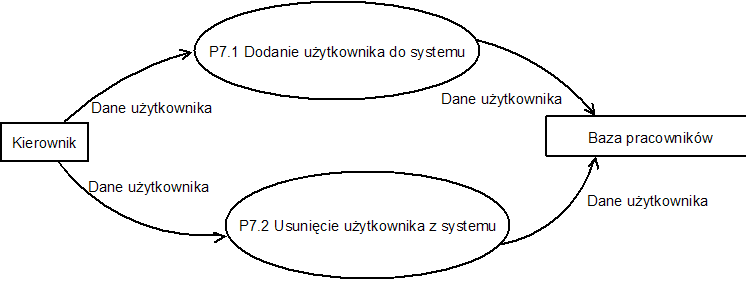
\includegraphics[width=1\textwidth]{gfx/dfd-2-7.png}
\caption{DFD - poziom 2.7 - Dodanie/usunięcie użytkownika systemu}
\end{figure}
\clearpage
\subsubsection{Poziom 2.8 - Wprowadzenie nowego towaru, usunięcie starego lub zmiana danych towarów}
\begin{figure}[h]
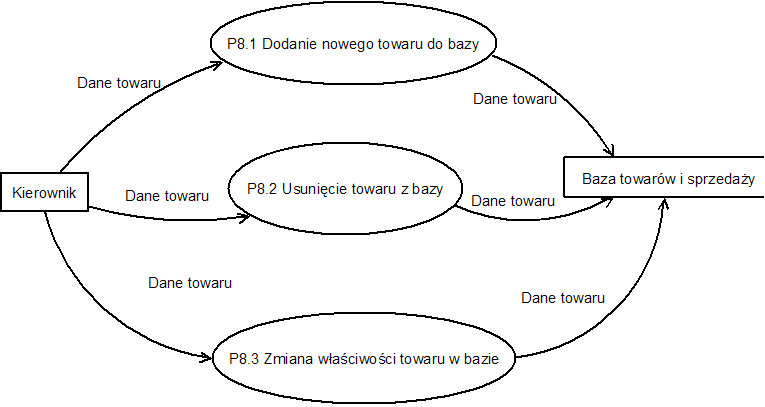
\includegraphics[width=1\textwidth]{gfx/dfd-2-8.png}
\caption{DFD - poziom 2.8 - Wprowadzenie nowego towaru, usunięcie starego lub zmiana danych towarów}
\end{figure}
\clearpage
\subsection{Opisy procesów}
\subsubsection{Proces P1 - Sprzedaż towaru}
\begin{description}
\item[Proces P1.1 - Zmniejszenie o~odpowiednią ilość stanu magazynu] ~\\*
Sprzedanie towaru musi skutkować zmniejszeniem, o~ilość adekwatną do ilości sprzedanego towaru, ilości danego towaru w~bazie danych. Próba sprzedania większej ilości towaru niż znajduje się w~magazynie, a~co za tym idzie w~bazie, skutkuje wyświetleniem komunikatu z~informacją o~niemożności zrealizowania transakcji i~zatrzymanie sprzedaży.
\item[Proces P1.2 - Wprowadzenie informacji o~sprzedaży do logu sprzedaży] ~\\*
Po dokonaniu sprzedaży towaru, informacje o~tym zdarzeniu należy zapisać do tablicy logów. Wpis taki powinien zawierać:
\begin{itemize}
\item numer salonu
\item identyfikator sprzedającego pracownika
\item identyfikator klienta o~ile klientowi wystawiana jest faktura
\item identyfikator towaru
\item ilość towaru
\item cena jednostkowa
\item data i~czas sprzedaży.
\end{itemize}
\item[Proces P1.3 - Pobieranie informacji o~produkcie]  ~\\*
Informacje potrzebne do dokonania transakcji należy pobrać z~bazy danych na podstawie kodu PLU przekazanego do systemu przez czytnik kodów kreskowych. W~szczególności z~bazy należy pobrać
\begin{itemize}
\item nazwę towaru
\item cenę jednostkową
\item dostępną ilość towaru
\item stawkę VAT
\end{itemize}
odpowiadające towarowi o~danym PLU.
\item[Proces P1.4 - Wystawienie faktury klientowi]  ~\\*
Sprzedawca dysponując danymi klienta sprawdza, czy klient o~takich danych jest już wprowadzony do systemu. Jeżeli tak, to potwierdza poprawność danych, koryguje je w~razie potrzeby i~wystawia fakturę dla tego klienta na kwotę i~towar zgodny ze sprzedanym. Jeżeli dane klienta nie znajdują się w~systemie, sprzedawca wprowadza dane klienta do systemu i~drukuje fakturę dla nowo utworzonego klienta.
\end{description}
\subsubsection{Proces P2 - Wprowadzenie dostawy}
\begin{description}
\item[Proces P2.1 - Dodanie towarów do stanu magazynowego] ~\\*
Pracownik, odbierając dostawę towaru, zwiększa ilość danego towaru w~bazie danych. Towar rozpoznawany jest za pomocą jego kodu kreskowego, tak więc zadanie pracownika ogranicza się od sczytania kodu PLU towaru i~wprowadzenia liczby dostarczonych sztuk. Informacja o~dodaniu towaru powinna być odnotowana w~logu magazynowym i~powinna zawierać:
\begin{itemize}
\item identyfikator saloniku
\item identyfikator pracownika przyjmującego i~wprowadzającego dostawę
\item identyfikator produktu
\item wielkość dostawy (ilość sztuk)
\item czas wprowadzenia dostawy
\end{itemize}
\item[Proces P2.2 - Wprowadzenie ceny towaru] ~\\*
W~przypadku kiedy dostarczony towar należy sprzedawać w~innej cenie niż cena wprowadzona w~systemie (np. prasa przyszła z~nadrukowaną inną ceną niż dotychczas) pracownik zmienia cenę danego towaru dla swojego salonu w~systemie. Informacja o~zmianie ceny jest odnotowywana w~bazie wraz z~informacją o~czasie zmiany oraz o~osobie dokonującej tej zmiany.
\item[Proces P2.3 - Dodanie kodu PLU do towaru] ~\\*
W~przypadku kiedy dostarczony towar ma kod PLU, nierozpoznawany przez system (czasami towar przychodzi z~nowym kodem PLU), pracownik wyszukuje towar w~bazie danych po jego nazwie, a~następnie dodaje nowy PLU dla tego towaru. PLU nowego towaru rozpoznawany jest za pomocą czytnika kodów kreskowych.
\end{description}
\subsubsection{Proces P3 - Przeglądanie statystyk salonu}
\begin{description}
\item[Proces P3.1 - Pobranie odpowiednich danych z bazy i~przetworzenie ich do prezentacji] ~\\*
Kierownik salonu oraz osoba zarządzająca siecią saloników mają możliwość przeglądania wybranego przez siebie rodzaju statystyk dotyczących funkcjonowania danego saloniku. Statystyki powinny być prezentowane w postaci wykresów słupkowych. Dostępne są następujące rodzaje statystyk:
\begin{description}
\item[Statystyki sprzedaży towaru] opisujące ilość sprzedanego wybranego towaru w ujęciu dziennym, miesięcznym lub rocznym, wraz z ilością sprzedanego towaru podana jest też wartość sprzedaży. Dodatkowo dostępna jest statystyka przedstawiająca rozkład ilości sprzedanego towaru w ujęciu miesięcznym, tygodniowym i dziennym w ustalonym okresie czasu (np. procentowy rozkład sprzedaży danego towaru w ciągu dnia z podziałem na godziny, biorąc pod uwagę ostatni miesiąc, albo procentowy rozkład sprzedaży w ciągu tygodnia z podziałem na dni tygodnia biorąc pod uwagę dane ze sprzedaży z ostatnich 25 dni.
\item[Statystyki sprzedaży] opisujące całkowitą ilość sprzedanego towaru w wyznaczonym okresie czasu, wartość tej sprzedaży, a także rankingi towarów wg. ilości sprzedanych sztuk oraz wartości tej sprzedaży.
\item[Statystyki zmian] opisujące sprzedaż (ilość, wartość) pogrupowane wg. godzin zmiany (poranna, popołudniowa, wieczorna) lub wg. pracowników z wybranego okresu czasu
\end{description}
Ponadto, możliwe jest przeglądanie raportów z pracy saloniku, w tym:
\begin{description}
\item[Raporty ze zmian] zawierające podsumowania kolejnych zmian pracowników
\item[Raporty dzienne] zawierające podsumowanie całodziennej działalności saloniku
\item[Raporty o zmianach cen] zawierające informacje o zmianach cen wprowadzonych przez pracownika przy odbieraniu dostawy
\end{description}
\end{description}
\subsubsection{Proces P4 - Przeglądanie statystyk globalnych}
\begin{description}
\item[Proces P4.1 - Pobranie odpowienich danych z bazy i~przetworzenie ich do prezentacji] ~\\*
Osoba zarządzająca siecią ma możliwość przeglądania statystyk wygenerowanych nie dla jednego salonu, lecz zagregowanych dla kilku saloników lub dla całej sieci. Format takich statystyk identyczny jest do formatu statystyk dla pojedynczego salonu. Ponadto dostępne są też statystyki porównawcze salonów, w tym:
\begin{description}
\item[Statystyki sprzedaży] opisujące wielkość i wartość sprzedaży saloniku w porównaniu z innymi oraz ranking najlepszych saloników
\item[Statystyki sprzedaży towarów] opisujące wielkość i wartość sprzedaży danego towaru w porównaniu z innymi salonikami w podanym okresie czasu
\end{description}
Ponadto, osoba zarządzająca ma wgląd do raportów wygenerowanych przez wszystkie saloniki, w szczególności do raportów informujących o zmianach cen wprowadzonych przez pracowników w czasie dostawy towaru.
\end{description}
\subsubsection{Proces P5 - Logowanie do systemu}
\begin{description}
\item[Proces P5.1 - Weryfikacja użytkownika] ~\\*
\end{description}
\subsubsection{Proces P6 - Nadawanie i przeglądanie uprawnień i danych użytkowników systemu}
\begin{description}
\item[Proces P6.1 - Pobieranie odpowiednich danych z bazy i przetworzenie ich do prezentacji] ~\\*
\item[Proces P6.2 - Nadanie określonych uprawnień wybranym pracownikom] ~\\*
\end{description}
\subsubsection{Proces P7 - Dodanie/usunięcie użytkownika systemu}
\begin{description}
\item[Proces P7.1 - Dodanie użytkownika do systemu] ~\\*
\item[Proces P7.2 - Usunięcie użytkownika z systemu] ~\\*
\end{description}
\subsubsection{Proces P8 - Wprowadzenie nowego towaru, usunięcie starego lub zmiana danych towarów}
\begin{description}
\item[Proces P8.1 - Dodanie nowego towaru do bazy] ~\\*
\item[Proces P8.2 - Usunięcie towaru z bazy bazy] ~\\*
\item[Proces P8.3 - Zmiana właściwości towaru w bazie] ~\\*
\end{description}